\chapter{State of the Art}

The broader DAA literature distinguishes between cooperative systems, where other traffic broadcasts its state, and non-cooperative systems, where the intruder must be sensed. Surveys on sense-and-avoid and UAS collision avoidance highlight that reliable perception, tracking, and conflict assessment remain central challenges for integrating unmanned aircraft into shared airspace \cite{fasano2016senseAvoid,skowron2019senseAvoidSmallUAS,pham2015collisionAvoidanceSurvey}.

\section{Sensor Modalities for Drone Detection}

Several studies have investigated the use of LiDAR for detecting small UAVs. Hammer et al.\ present a comprehensive overview of the challenges and opportunities associated with LiDAR-based drone detection \cite{hammer2018potentialLidarUAV,hammer2018lidarSmallUAVs}. They highlight that small UAVs are difficult to detect because they generate only a few LiDAR returns, especially at long range, and that their appearance can be similar to birds or other airborne objects. They proved that detection and tracking performance depends strongly on the LiDAR scanning rate, resolution, range, and observation geometry of the employed sensor system.
Dogru and Marques address the data-sparsity problem more explicitly by investigating drone detection when the target generates too few LiDAR returns for conventional dense point-cloud processing \cite{dogru2022sparseLidarDrone}.

An important step toward reproducible multimodal evaluation is provided by the MMAUD dataset. MMAUD combines stereo imagery, two three-dimensional LiDAR sensors with different fields of view, millimeter-wave radar, and acoustic arrays for drone detection, tracking, classification, and trajectory estimation \cite{yuan2024mmaud}. Drone positions are referenced using a Leica multi-station that tracks a prism mounted on the target UAV, providing a common spatial reference for the recorded modalities. The dataset is particularly relevant because it moves beyond image-only detection and includes both geometric measurements and three-dimensional target trajectories. Although MMAUD represents a central benchmark for multimodal ground-based drone perception, it does not address the continuously changing geometry and ego-motion associated with an airborne host platform.

The closest identified work to an air-to-air LiDAR setting is presented by Manduhu et al.\ \cite{manduhu2023airborneSenseDetect}. Their contribution is the design of a system that mounts a LiDAR and onboard processing hardware on a monitoring drone to detect and localize other drones during close-proximity operations. The authors demonstrate the proof of concept for data-driven LiDAR-based drone detection and tracking but do not publish their dataset or provide detailed evaluation results of model training and performance.

The reviewed literature shows that LiDAR and multimodal sensing can support data-driven three-dimensional drone detection and trajectory estimation. However publicly available datasets are limited and focus on ground based detection, with airborne LiDAR-data completely missing. Particularly for helicopter DAA, there is a need for adressing airborne scenarios and providing a public dataset and benchmark.

\begin{figure}[htbp]
    \centering
    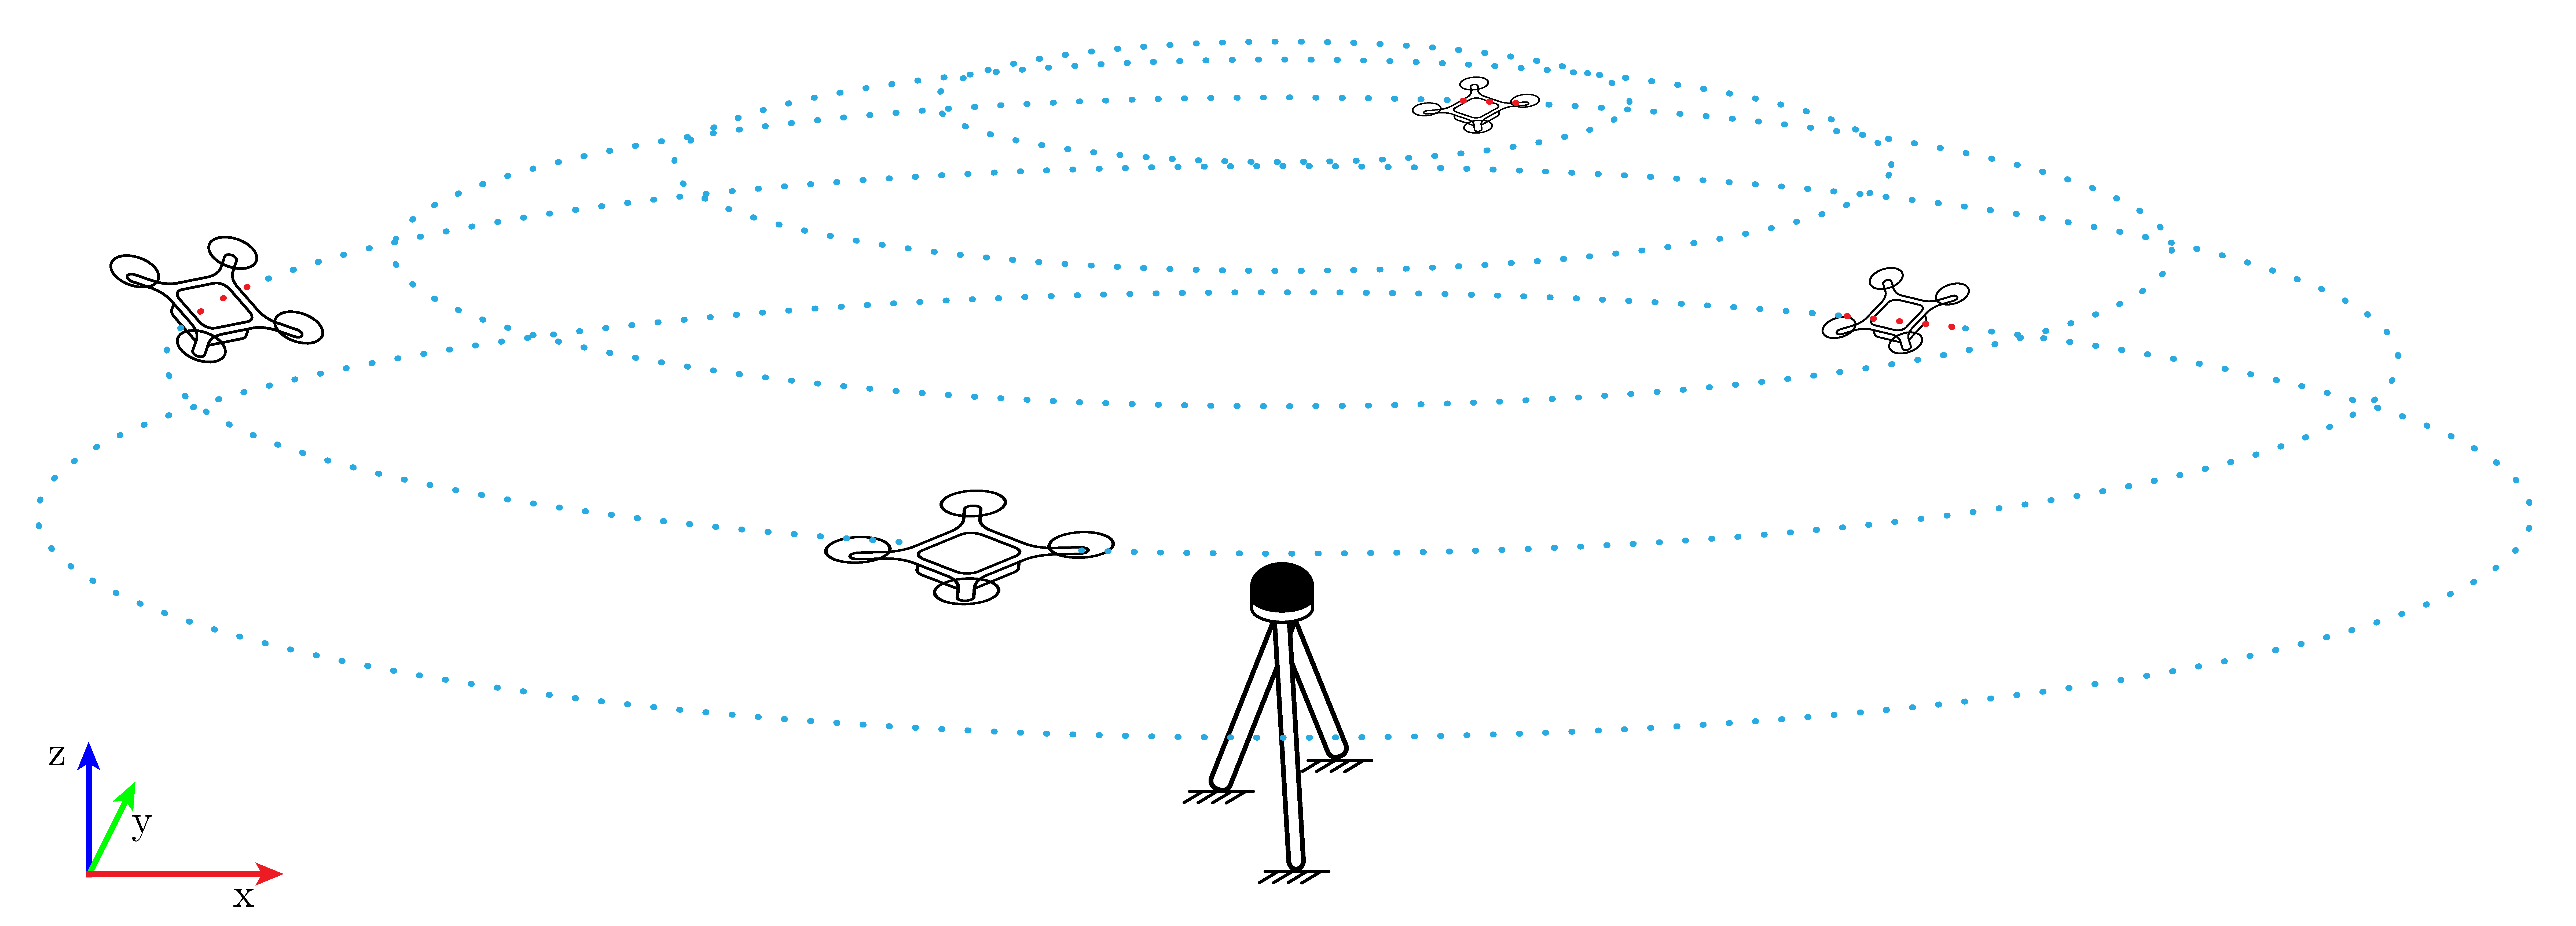
\includegraphics[width=\textwidth]{images/data_gen_ground.pdf}
    \caption{Ground-based spherical LiDAR for UAV data acquisition and detection as deployed for the MMAUD dataset \cite{yuan2024mmaud}. A LiDAR sensor is mounted on a tripod and records the target drones from a fixed position. Regarding helicopter DAA, this setup does not represent the geometry an airborne host platform.}
    \label{fig:data_gen_drone}
\end{figure}

\section{3D Object Detection}

Conventional LiDAR-based detection commonly relies on background subtraction and point-cloud clustering. After removing static scene elements, nearby measurements are grouped into clusters that may represent an object so that objects can be distinguished \cite{hammer2018lidarSmallUAVs,dogru2022sparseLidarDrone,liang2024unsupervisedLidarUAVTrajectories,seidaliyeva2025lidarUAVDetection}. These methods fast to deploy and require no annotated training data. However, their performance depends strongly on manually tuned thresholds and a stable background, making them difficult to apply when both the sensor platform and the target are moving. 

Data-driven methods learn geometric features and directly predict object classes and oriented three-dimensional bounding boxes. Existing LiDAR detectors can be broadly distinguished according to whether they process individual points, three-dimensional voxels, or vertically extended pillars. Point-based model-architectures derived from PointNet and PointNet++ preserve the precise coordinates of the measured points during object detection \cite{qi2017pointnet,qi2017pointnetpp}. This is beneficial for accurate localization, but processing irregular point sets is computationally very expensive.

Voxel-based methods convert the irregular point cloud into a regular three-dimensional grid. VoxelNet introduced an end-to-end architecture in which features are learned within individual voxels and processed using three-dimensional convolutions \cite{zhou2018voxelnet}. This representation preserves spatial structure along all three axes, but its inference time and memory requirements increase rapidly with the voxel resolution. Hybrid approaches such as SECOND \cite{yan2018second}, Centerpoint \cite{yin2021centerpoint} and PV-RCNN \cite{shi2020pvrcnn} reduce the models' computational cost by restricting convolution operations only to occupied voxels or combining sparse voxel features with point-based set abstraction or by representing objects through their centers and regressing their dimensions.
Within the highly constrained computational budgets of airborne perception, voxel-based methods may nevertheless remain too slow for real-time deployment. 

Pillar-based detectors prioritize computational efficiency by discretizing only the horizontal plane. PointPillars groups all points within a vertical column into a learned pillar feature, and processes the result using only two-dimensional convolutions \cite{lang2019pointpillars}. However, while the input features include the point height and the detection head regresses the vertical position and dimensions of the bounding box, the vertical distribution of points is compressed into a single feature per horizontal cell.
This 3D object detector was designed around autonomous driving scenarios, where vehicles, pedestrians, and cyclists are usually associated with a road surface and occur within a restricted vertical region. While PillarNet offers fast inference, the vertical compression may cause localization errors for aerial targets, which usually occur at arbitrary elevations.

Manduhu et al.\ adapted PointPillars to their air-to-air scenario by extending the vertical detection range and introducing anchors at different elevations \cite{manduhu2023airborneSenseDetect}. This demonstrates that pillar-based detectors can be configured to predict targets at different altitudes. Still, it remains necessary to determine whether the vertical compression inherent in pillar-based processing causes systematic detection or localization errors for sparse aerial targets, and whether explicit vertical encoding, hybrid voxel--pillar features, or temporal evidence can address these errors without losing the runtime advantages required for airborne deployment.

\section{Helicopter DAA, Conflict Assessment and Dynamic Avoidance Planning}

DAA describes the complete process from observing another aircraft to determining and executing an appropriate response. The Literature agrees on four core DAA-stages perception, conflict assessment, resolution generation, and avoidance maneuver execution \cite{kuchar2000conflictReview,fasano2016senseAvoid,riedel2025daaStandards}. 

\begin{figure}[htbp]
    \centering
    
\includegraphics[width=\textwidth]{images/DAA_flow_diagram.pdf}
    \caption{Flow diagram of the helicopter DAA process. The perception system provides estimates of the intruder's relative position and velocity. Based on these estimates, the conflict assessment stage determines whether a separation violation is likely to occur. If a conflict is detected, the resolution generation stage computes an avoidance maneuver that is feasible for the host aircraft. Finally, the avoidance maneuver is executed by the flight-control system.}
\end{figure}

First a perception system provides estimates of the intruder's relative position and velocity. Details on the These estimates are then used to determine whether the predicted trajectories violate a required separation and whether an avoidance maneuver is necessary. The precision of the intruders estimated relative state therefore directly affects all subsequent stages of DAA.

Conflict assessment is generally based on the projected relative motion between the two aircraft. Deterministic methods extrapolate the current position and velocity to calculate the time and distance to the closest point of approach. Probabilistic approaches additionally account for uncertainty in the estimated trajectories and determine the likelihood of a separation violation \cite{paielli1997conflictProbability,prandini2000probabilisticConflict}. This is particularly relevant for non-cooperative drones because their position and velocity must be estimated from onboard measurements. Consequently, a reliable conflict assessment must consider both, the predicted encounter geometry and the uncertainty associated with the prediction.

Once a conflict has been identified, the resolution stage generates a maneuver that avoids the intruder while remaining feasible for the host aircraft. Older geometric methods such as velocity obstacles \cite{fiorini1998velocityObstacles} and collision cones \cite{chakravarthy1998collisionCone} identify relative velocities that would result in a future collision and provide computationally efficient avoidance directions. However, these methods traditionally do not account for flight-dynamics. Model predictive control (MPC) addresses this limitation by considering vehicle dynamics while optimizing for future trajectories. Hence, MPC-based methods have been applied to UAV avoidance of moving obstacles and have also been combined with motion prediction from noisy measurements \cite{lindqvist2020dynamicObstacleMPC,olcay2024dynamicObstacleForecast}.

Alexej Dikarew proposed a sampling-based MPC method in \cite{dikarew2024helicopterMPCA} that predicts helicopter trajectories using a simplified six-degree-of-freedom model and selects a maneuver according to collision risk and deviation from the intended flight path. His approach demonstrated real-time avoidance in simulations. However, the  considered obstacles were stationary at predefined locations with sensor-based target detection not being included in the framework.

In \cite{whalley2014autonomousBlackHawk}, real-world experiments with the RASCAL JUH-60A have demonstrated the integration of onboard sensing, risk-aware obstacle mapping, and trajectory generation for autonomous helicopter navigation. 

Recent work has begun to connect onboard perception with aviation collision-avoidance logic. Crippa et al.\ combined radar and infrared sensing, target tracking, and an Airborne Collision Avoidance System (ACAS) -based resolution function for non-cooperative targets in simulation \cite{crippa2025acasNonCooperative}. This demonstrates how perception outputs can be propagated through conflict assessment to avoidance guidance. Nevertheless, here, the host vehicle was an UAV rather than a conventional helicopter, and the influence of perception uncertainty was not examined.

Overall, the individual components required for helicopter DAA (target tracking, probabilistic conflict assessment, moving-obstacle prediction with MPC, constrained maneuver generation, autonomous real helicopter flight) are established, but are evaluated separately or with the exact obstacle state supplied to the planner. The effects of data-driven drone detection methods on encounter-risk assessment and collision-avoidance planning remain unexplored.

\section{Research Gap}

A practical challenge in LiDAR-based drone perception is the scarcity of suitable datasets. Large public 3D detection datasets focus mostly on autonomous driving, while datasets for small airborne drone detection with LiDAR are limited. Synthetic data can help address this problem by enabling controlled variation of sensor properties, drone geometry, trajectories, ranges, and environmental conditions. However, synthetic data introduces a simulation-to-reality gap. Dieter et al.\ study this gap for deep-learning-based drone detection and show that synthetic data must be carefully designed and validated to support real-world generalization \cite{dieter2023simulationRealityGap}. Recent airborne LiDAR work also uses simulation and digital-twin concepts to generate training data for drone detection \cite{manduhu2023airborneSenseDetect}.

For this dissertation, synthetic data is relevant in two ways. First, it enables systematic generation of sparse LiDAR drone encounters, including rare or safety-critical scenarios that are difficult to collect experimentally. Second, it allows controlled evaluation of tracking and trajectory prediction methods under known ground truth. Nevertheless, the resulting methods must be assessed with respect to generalization. A benchmark should therefore separate training and unseen test scenarios and should report not only detection accuracy, but also tracking continuity, velocity estimation, future position error, and conflict-relevant quantities.

The reviewed literature shows substantial progress in DAA systems, LiDAR-based 3D detection, multi-object tracking, and trajectory prediction. However, the specific problem of tracking and predicting non-cooperative drones from sparse airborne LiDAR remains insufficiently addressed. Existing 3D detectors are largely optimized for ground-based autonomous-driving scenarios. Existing drone detection work often focuses on per-frame detection or ground-based counter-UAV sensing. Existing trajectory prediction methods frequently assume cleaner trajectory observations than are available from sparse LiDAR detections.

The central research gap is therefore the lack of an integrated, safety-oriented pipeline that converts sparse airborne LiDAR measurements of small non-cooperative drones into temporally stable tracks and short-horizon trajectory predictions. Addressing this gap requires combining LiDAR-based detection, uncertainty-aware tracking, and trajectory forecasting in a way that is suitable for helicopter detect-and-avoid scenarios. The proposed dissertation will investigate this connection and evaluate how temporal integration can improve the reliability of drone state estimation beyond single-frame detection.
